\documentclass[authoryear, 12pt,5p, times]{elsarticle}
\usepackage[hypcap]{caption}
\usepackage{float}
\usepackage{amsmath}
\usepackage[hidelinks]{hyperref} 
 \usepackage{gensymb}
\usepackage{subcaption}
\usepackage{url}
%\renewcommand\thefootnote{\fnsymbol{\dagger}}
\usepackage[symbol*]{footmisc}
\begin{document}
%\footnote{This is a footnote}
\begin{frontmatter}
\title{Astronomical Spectroscopy: Detecting light with a CCD}
\author{\today \\ \quad \\Jung Lin (Doris) Lee\\ dorislee@berkeley.edu\\Group partners: Jennifer Ito, Manuel Silvia\\Prof. James Graham, UGSI Heechan Yuk, Isaac Domagalski}
	\begin{abstract}
    %key objective, method, principle conclusion 
	ABSTRACT HERE
	\end{abstract}
\end{frontmatter}
\section{Introduction\label{intro}}
Spectra important chemical composition 
spectra provides composition detail to planetary bodies , stars, also the surrounding medium 
analysis
Recent development in +++++ Baryon Oscillation Spectroscopic Survey (BOSS; Dawson et al.)

is a result of each CCD pixel's different sensitivity to photon
\begin{figure}
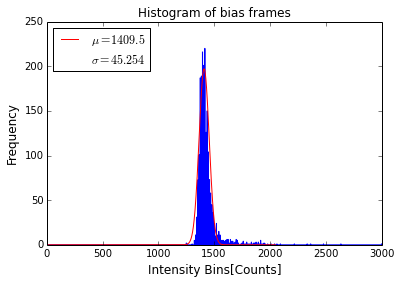
\includegraphics[width=0.5\textwidth]{figures/bias_histo}
\caption{We took a dataset of 1s integration time bias frames by placing the red cap on the spectrometer and in a black bag. A histogram of dark counts is fitted to a Gaussian. The variance of the distribution relates to the read noise and gain of the spectrometer \citep{ccd_handbook}.}
\end{figure}
\section{Experiment and }
\subsection{Spectra property and comparison for different sources}
\section{Data Reduction}
	\subsection{Automated centroid algorithm}
	find the local maxima and minima by comparing subsequent data points and testing the boolean condition of function increasing or decreasing.
We attempted to create a automated centroid algorithm by selecting the centroid that we actually care about, we impose two conditions:1. the data range that we use to calculaute the centroid must be the region wihtin a min-max-min group, Since almost a large number of datapoint will satisfy thiscondition and it doesn't tell us teh intensity difference between the local max and min are, so we impose a second condition that the difference must be greater than 10\% of the difference between maximum datapoint of the first dataset and the minimum datapoint (so that the offset is considered in). The 10\% was chosen because of the quality of the centroid result that it produces.
\begin{figure}
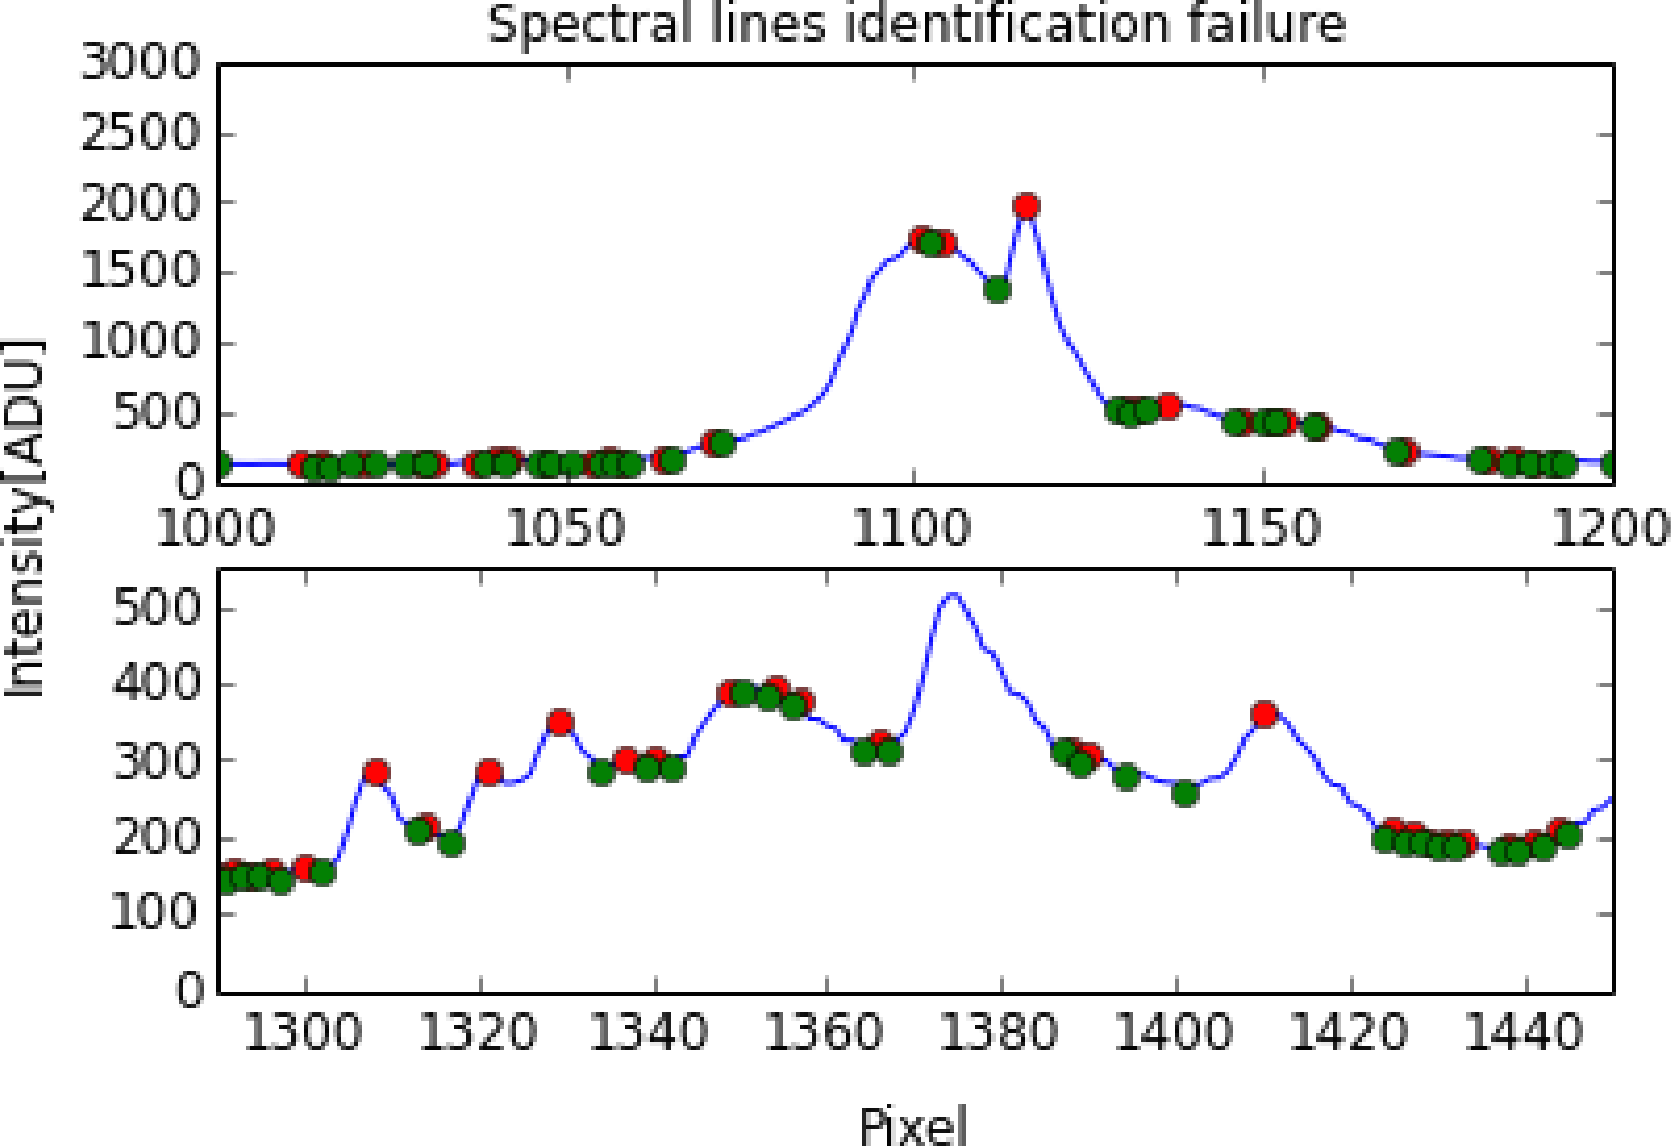
\includegraphics[width=0.45\textwidth]{figures/fail}
\caption{Top: The closely spaced extremum at around the 1100th pixel results in a small difference value between the local minimum and maximum. Therefore, it was not detected by the algorithm. Bottom: The extremum finding algorithm did not detect the maximum at around pixel 1380 in its  first step.}
\end{figure}
	%the algorithm is robust as it is proven to find accurate centroid on a test data of 10000 sample (do later)
	The alogirthim was not very robust as it is unable pick out spectral lines that lied between consecutive extremas such as the ones on pixel 1115 and 1374. Despite varying the percentage cut, it was unable to identify features that showed relative difference such as 314 but only measured the absolute differences, which is hard to account for with such great differences.
\begin{figure}
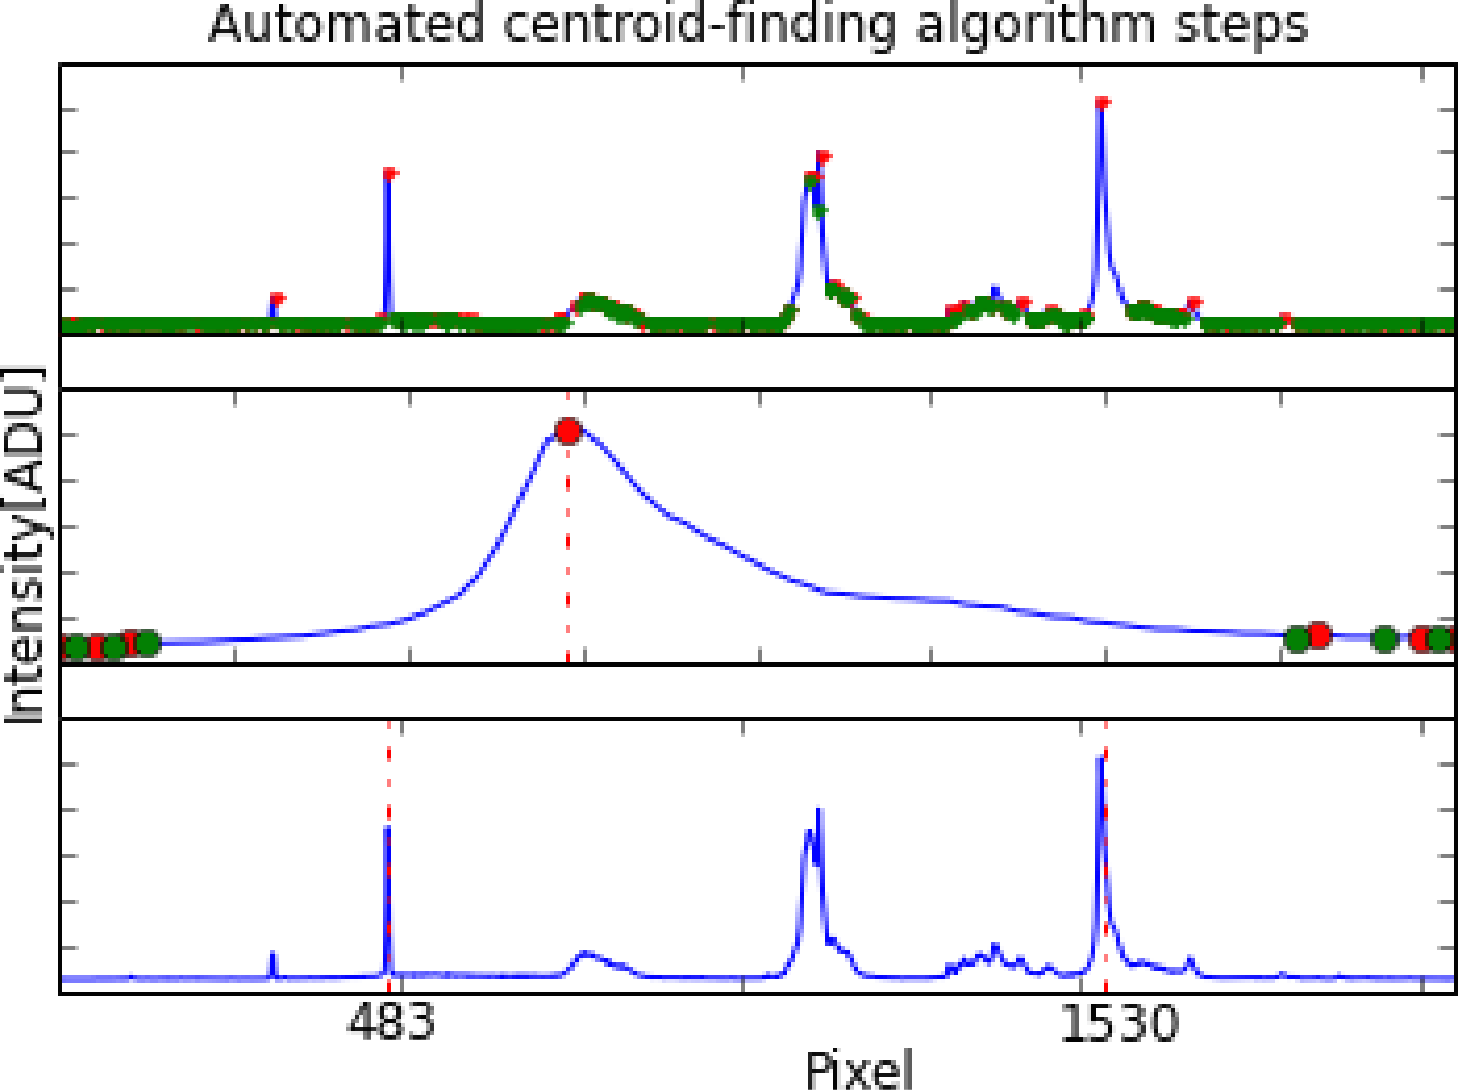
\includegraphics[width=0.45\textwidth]{figures/steps}
\caption{Graphical representation of how the automated algorithm works. Top: Identifying all the extremum of the dataset. Red marker denotes local maximum; green denotes local minimum. Middle: Applying criteria to select suitable ranges as shown in middle plot, using this sliced dataset to obtain the centroid values (dashed). Bottom: Resulting centroid list misses some important spectral feature picked out by the eyeball-estimation method shown in Fig. (\textbf{REF!!!!}).} 
\end{figure}
	\subsection{Systematic Effects}
	 \subsection{Natural Broadening Effect}
 As seen in Fig. (LABEL HERE) the spectral lines are not perfect sharp Dirac Delta functions. This broadening is due to several physical phenomena, one reason is the natural line width caused by the measurement uncertainty inherent from quantum mechanics. Another more dominant effect is due to Doppler shift from the thermal velocity of the atoms. The distribution of the atomic thermal velocity is governed by the Boltzmann distribution. This Doppler-shifted velocity distribution propagates to our intensity measurement, which can then be rearranged into a Gaussian form. The broadening effect is chracterized by the variance of this new distribution as shown in  Eq. \ref{doppler_var},
 \begin{equation}\label{doppler_var}
\sigma_f = \sqrt{\frac{kT}{mc^2}}f_0
 \end{equation}
 where T is the temperature, m is the mass of the atom, $f_0$ is the frequency when atom is stationary, c is the speed of light and k is the Boltzman factor.
 
 \subsection{Dark Counts}
 
source of error: 
- ununiform pixels(REF dark counts)
- multiple mixed source since roomlight not closed when taking data, so slight traces of other sources in our pure data like neon...etc
 
\section{Conclusion}

Possible extension to this project may be to try conducting a basic flat-field correction to the detector. One way to do this to shine bright light uniformly on the detector to see the response of each pixel.  The exposure time needs to be short so that the CCD is not saturated. We can also try to measure maximum ranges at which CCD is sensitive and linear.
\bibliography{references}
 %\bibliographystyle{abbrvnat}
%\bibliographystyle{apalike}
%\bibliographystyle{plainnat}
%\bibliographystyle{unsrtnat}
\bibliographystyle{elsarticle-harv}
Haken, Hermann and Wolf, Hans Christolph, The Physics of Atoms and Quanta, 5th Ed., Springer-Verlag, 1996.
\end{document}
